% Figure for MATH 591 §76 (Lecture 30), generated by courses/591/new/2026-11-13-L30/gen.py
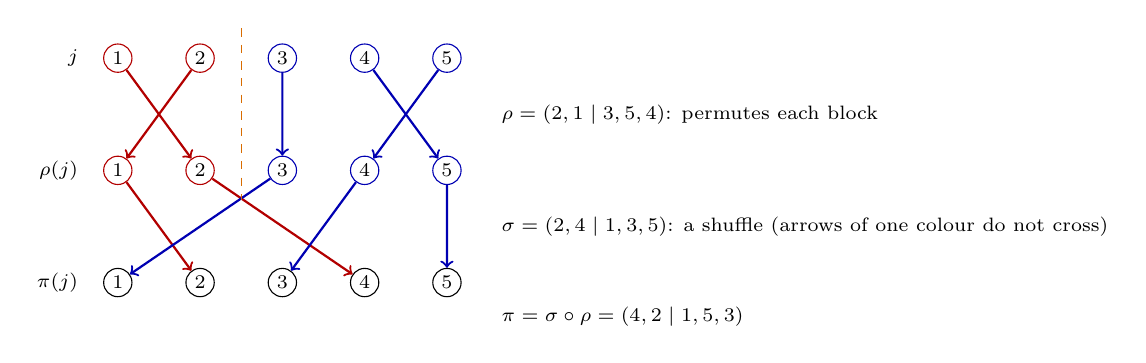
\begin{tikzpicture}[scale=0.95]
\node[circle, draw=red!70!black, inner sep=1.5pt, font=\scriptsize] (n01) at (0.00,3.0) {$1$};
\node[circle, draw=red!70!black, inner sep=1.5pt, font=\scriptsize] (n02) at (1.10,3.0) {$2$};
\node[circle, draw=blue!70!black, inner sep=1.5pt, font=\scriptsize] (n03) at (2.20,3.0) {$3$};
\node[circle, draw=blue!70!black, inner sep=1.5pt, font=\scriptsize] (n04) at (3.30,3.0) {$4$};
\node[circle, draw=blue!70!black, inner sep=1.5pt, font=\scriptsize] (n05) at (4.40,3.0) {$5$};
\node[circle, draw=red!70!black, inner sep=1.5pt, font=\scriptsize] (n11) at (0.00,1.5) {$1$};
\node[circle, draw=red!70!black, inner sep=1.5pt, font=\scriptsize] (n12) at (1.10,1.5) {$2$};
\node[circle, draw=blue!70!black, inner sep=1.5pt, font=\scriptsize] (n13) at (2.20,1.5) {$3$};
\node[circle, draw=blue!70!black, inner sep=1.5pt, font=\scriptsize] (n14) at (3.30,1.5) {$4$};
\node[circle, draw=blue!70!black, inner sep=1.5pt, font=\scriptsize] (n15) at (4.40,1.5) {$5$};
\node[circle, draw=black, inner sep=1.5pt, font=\scriptsize] (n21) at (0.00,0.0) {$1$};
\node[circle, draw=black, inner sep=1.5pt, font=\scriptsize] (n22) at (1.10,0.0) {$2$};
\node[circle, draw=black, inner sep=1.5pt, font=\scriptsize] (n23) at (2.20,0.0) {$3$};
\node[circle, draw=black, inner sep=1.5pt, font=\scriptsize] (n24) at (3.30,0.0) {$4$};
\node[circle, draw=black, inner sep=1.5pt, font=\scriptsize] (n25) at (4.40,0.0) {$5$};
\draw[->, red!70!black, thick] (n01) -- (n12);
\draw[->, red!70!black, thick] (n12) -- (n24);
\draw[->, red!70!black, thick] (n02) -- (n11);
\draw[->, red!70!black, thick] (n11) -- (n22);
\draw[->, blue!70!black, thick] (n03) -- (n13);
\draw[->, blue!70!black, thick] (n13) -- (n21);
\draw[->, blue!70!black, thick] (n04) -- (n15);
\draw[->, blue!70!black, thick] (n15) -- (n25);
\draw[->, blue!70!black, thick] (n05) -- (n14);
\draw[->, blue!70!black, thick] (n14) -- (n23);
\draw[orange!85!black, dashed] (1.65,3.4) -- (1.65,1.1);
\node[font=\scriptsize, anchor=west] at (5.0,2.25) {$\rho = (2, 1 \mid 3, 5, 4)$: permutes each block};
\node[font=\scriptsize, anchor=west] at (5.0,0.75) {$\sigma = (2, 4 \mid 1, 3, 5)$: a shuffle (arrows of one colour do not cross)};
\node[font=\scriptsize, anchor=west] at (5.0,-0.45) {$\pi = \sigma \circ \rho = (4, 2 \mid 1, 5, 3)$};
\node[font=\scriptsize, anchor=east] at (-0.4,3.0) {$j$};
\node[font=\scriptsize, anchor=east] at (-0.4,1.5) {$\rho(j)$};
\node[font=\scriptsize, anchor=east] at (-0.4,0.0) {$\pi(j)$};
\end{tikzpicture}
